\documentclass[aspectratio=169,
hyperref={colorlinks,urlcolor=blue}
]{beamer}


%\usetheme{Pittsburgh}
\usetheme{default}
\usepackage{colortbl}%colored tables
%For using helvetica font:
\usepackage[scaled]{helvet}
\usepackage[T1]{fontenc}
\renewcommand\familydefault{\sfdefault}
\urlstyle{same} %sets the fonts for urls
\usepackage{pdfpages}
\usepackage{siunitx}
\usepackage{caption}
\usepackage{pifont}%for dings
\usepackage{pgfplots}%for 3d plotting
\pgfplotsset{compat = newest}
\usepackage{mathtools}%box in align env \Aboxed
\usepackage[american,smartlabels]{circuitikz}%for drawing circuits
\usepackage{multimedia}
\usepackage{animate}
\usepackage{xcolor}


\usetikzlibrary{arrows}
\usetikzlibrary {3d} 
\usetikzlibrary{decorations.markings, math}
\usetikzlibrary{intersections, pgfplots.fillbetween}
\usetikzlibrary {shapes.geometric} 


%\definecolor{myblue}{RGB}{5, 34, 150}
\definecolor{myblue2}{RGB}{5, 34, 150}
\definecolor{myblue}{RGB}{0,36,82}
\definecolor{myred}{RGB}{207, 2, 13}
\definecolor{mygreen}{RGB}{0, 158, 11}
\definecolor{myyellow}{RGB}{220,220,0}
\definecolor{qblue}{RGB}{0,36,82}
\definecolor{qgold}{RGB}{250,189,15}
\definecolor{qred}{RGB}{185,14,49}
\definecolor{cblue}{rgb}{0.13, 0.67, 0.8}
\definecolor{corange}{rgb}{0.8, 0.34, 0.0}
\definecolor{cpurple}{rgb}{0.54, 0.29, 0.42}

%%%%%%%%%%%% General settings
\setbeamercolor{frametitle}{fg=black}
\setbeamercolor{title}{fg=black}
\setbeamercolor{author}{fg=myblue2}

\beamertemplatenavigationsymbolsempty %no navigation controls at bottom of slides
%\setbeamertemplate{footline}[frame number]
\usefonttheme{professionalfonts} 
\setbeamerfont{title}{series=\bfseries,parent=structure}
\setbeamerfont{frametitle}{series=\bfseries,parent=structure}

%%%%%%%%%%%%Lists
\setbeamertemplate{itemize item}[circle] %{\color{myblue}$\circ$}
\setbeamertemplate{itemize subitem}{\color{myblue2}$\circ$}
\setbeamertemplate{itemize subsubitem}{\color{myblue2}$\cdot$}
\setbeamercolor{itemize item}{bg=myblue2,fg=myblue2}
\setbeamercolor{enumerate item}{bg=myblue2,fg=myblue2}
%%%%%%%%%%%%%%%%%%%%%%%%%%%%

%%%%%%%%%%%%Blocks
\setbeamertemplate{blocks}[rounded]
%Default block
\setbeamercolor{block title}{bg=myblue2, fg=white}
\setbeamercolor{block body}{bg=myblue2!10}
\setbeamerfont{block body}{size=\scriptsize}
\setbeamerfont{block title}{size=\scriptsize}
%Alert block
\setbeamercolor{block title alerted}{bg= myblue2, fg=white}
\setbeamercolor{block body alerted}{bg=myblue2!10}
\setbeamerfont{block body alerted}{size=\scriptsize}
\setbeamerfont{block title alerted}{size=\scriptsize}
%example block
\setbeamercolor{block title example}{bg=mygreen, fg=white}
\setbeamercolor{block body example}{bg=mygreen!10}
\setbeamerfont{block body example}{size=\scriptsize}
\setbeamerfont{block title example}{size=\scriptsize}
%%%%%%%%%%%%%%%%55


%%%%%%%%%%%%Figures and captions
\captionsetup{font=scriptsize,labelfont=scriptsize}
%\setbeamertemplate{caption}{\raggedright\insertcaption\par}
\newenvironment{capfig}[3]{\begin{figure}\includegraphics[width=#1\textwidth]{#2}\caption*{\textit{#3}}\end{figure}}{}

%\makeatother
%\setbeamertemplate{footline}
%{
%  \leavevmode%
%  \hbox{%
%  \begin{beamercolorbox}[wd=.4\paperwidth,ht=2.25ex,dp=1ex,center]{author in head/foot}%
%    \usebeamerfont{author in head/foot}\insertshortauthor
%  \end{beamercolorbox}%
%  \begin{beamercolorbox}[wd=.6\paperwidth,ht=2.25ex,dp=1ex,center]{title in head/foot}%
%    \usebeamerfont{title in head/foot}\insertshorttitle\hspace*{3em}
%    \insertframenumber{} / \inserttotalframenumber\hspace*{1ex}
%  \end{beamercolorbox}
%  }%
%  \vskip0pt%
%}
%\makeatletter

\makeatother
\setbeamertemplate{footline}
{
  \leavevmode%
  \hbox{%
\begin{beamercolorbox}[wd=.27\paperwidth,ht=2.25ex,dp=1ex,center]{author in head/foot}%
    \color{black}{\insertinstitute}
\end{beamercolorbox}
  \begin{beamercolorbox}[wd=.27\paperwidth,ht=2.25ex,dp=1ex,center]{author in head/foot}%
    \color{black}{\inserttitle}
  \end{beamercolorbox}%
  \begin{beamercolorbox}[wd=.27\paperwidth,ht=2.25ex,dp=1ex,center]{title in head/foot}%
    \color{black}{\insertshortauthor}
  \end{beamercolorbox}
  \begin{beamercolorbox}[wd=.27\paperwidth,ht=2.25ex,dp=1ex,center]{title in head/foot}%
    \hspace{.28\paperwidth}\color{black} \insertframenumber{} / \inserttotalframenumber\hspace*{1ex}
  \end{beamercolorbox}
  }%
  \vskip0pt%
}
\makeatletter

\setbeamertemplate{title page}
{
  \begin{tikzpicture}[remember picture,overlay]
    \def\barh{4}%15
  
    \draw[color=myblue2,line width=\barh] ([yshift=-0.5*\barh]current page.north west) -- ([yshift=-0.5*\barh,xshift=-0.67\paperwidth]current page.north east);
    \draw[color=myblue2,line width=\barh] ([yshift=-0.5*\barh,xshift=-0.67\paperwidth]current page.north east) -- ([yshift=-0.5*\barh,xshift=-0.34\paperwidth]current page.north east);
    \draw[color=myblue2,line width=\barh] ([yshift=-0.5*\barh,xshift=-0.34\paperwidth]current page.north east) -- ([yshift=-0.5*\barh]current page.north east); 
  
    \draw[color=myblue2,line width=\barh] ([yshift=0.5*\barh]current page.south west) -- ([yshift=0.5*\barh,xshift=-0.67\paperwidth]current page.south east);
    \draw[color=myblue2,line width=\barh] ([yshift=0.5*\barh,xshift=-0.67\paperwidth]current page.south east) -- ([yshift=0.5*\barh,xshift=-0.34\paperwidth]current page.south east);
    \draw[color=myblue2,line width=\barh] ([yshift=0.5*\barh,xshift=-0.34\paperwidth]current page.south east) -- ([yshift=0.5*\barh]current page.south east);
    %\node[left] at (current page.east) {
    %
\includegraphics[scale=0.1]{figures/coverpage}
    %};
  \end{tikzpicture}
  
  \usebeamerfont{title}\usebeamercolor[fg]{title}\inserttitle\par
  \usebeamerfont{subtitle}\usebeamercolor[fg]{subtitle}\insertsubtitle\par
  \vspace{2cm}
  \usebeamerfont{author}\usebeamercolor[fg]{author}\insertauthor\par
  \usebeamerfont{institute}\usebeamercolor[fg]{author}\insertinstitute\par
  \usebeamercolor[fg]{author}\par
  \usebeamercolor[fg]{titlegraphic}\inserttitlegraphic

} 

\setbeamertemplate{frametitle}{%
    \nointerlineskip%
        \par\hspace*{-\dimexpr0.5\paperwidth-0.5\textwidth}\textcolor{myblue2}{\rule{0.33\paperwidth}{6pt}}\textcolor{myblue2}{\rule{0.33\paperwidth}{6pt}}\textcolor{myblue2}{\rule{0.34\paperwidth}{6pt}} 
    \begin{beamercolorbox}[wd=\paperwidth,ht=0.75cm,dp=0.6ex]{frametitle}
        \hspace*{0.5cm}\strut\usebeamerfont{frametitle}\insertframetitle\strut
        %\hrule
    \end{beamercolorbox}%
    %%Line below:
%\par\hspace*{-\dimexpr0.5\paperwidth-0.5\textwidth}\textcolor{myblue}{\rule{\paperwidth}{0.4pt}}
     % <-- calculation of left margin width + rule
     %\textcolor{red}{\noindent\rule{\paperwidth}{2pt}}
}


%%%%%%%%%%%%Frame templates

%Slide with title
\newenvironment{titleframe}[1]
{\begin{frame}\frametitle{#1}\end{frame}}
{}

%Slide with title and itemize list:
\newenvironment{bulletframe}[1]
{\begin{frame}{#1} \itemize}
{\enditemize \end{frame}}

%Slide with two columns 50/50
\newenvironment{twocolframe}[3]
{\begin{frame}{#1}
 \begin{columns}[T]
 \column{0.5\textwidth}#2
 \column{0.5\textwidth}#3
 \end{columns}\end{frame}}{}

%Slide with two columns 60/40 <<<<<<<<<<<<<<<<<<<<<<  This one!
\newenvironment{twocolframesf}[3]
{\begin{frame}{#1}
 \begin{columns}[T]
 \column{0.6\textwidth}#2
 \column{0.4\textwidth}#3
 \end{columns}\end{frame}}{}
 
%Slide with two columns 70/30
\newenvironment{twocolframest}[3]
{\begin{frame}{#1}
 \begin{columns}[T] 
 \column{0.7\textwidth}#2
 \column{0.3\textwidth}#3
 \end{columns}\end{frame}}{} 
 
%Slide with two columns 40/60
\newenvironment{twocolframefs}[3]
{\begin{frame}{#1}
 \begin{columns}[T] 
 \column{0.4\textwidth}#2
 \column{0.6\textwidth}#3
 \end{columns}\end{frame}}{}
 
%Slide with two columns 70/30
\newenvironment{twocolframets}[3]
{\begin{frame}{#1}
 \begin{columns}[T] 
 \column{0.3\textwidth}#2
 \column{0.7\textwidth}#3
 \end{columns}\end{frame}}{} 

 
%Colloquium speaker (title, abstract, picture file, speaker name)
\newenvironment{colloquium}[5]
{
\begin{frame}{Colloquium: Friday 1:30pm in Stirling A}
\begin{columns}[T] 
 \column{0.8\textwidth}
 \textbf{#1}\\
 #2
 \column{0.2\textwidth}
 \capfig{#3}{#4}{#5}
 \end{columns}
\end{frame}
}
{} 

%%%%%%%%%%%%%Set Hyperref colors


\hypersetup{
  colorlinks=true,
  linkcolor=blue,    
  urlcolor=blue,     
  citecolor=blue      
}
%%%%%%%%%%%%%TOC bolding
\setbeamerfont{section in toc}{series=\bfseries}



%Frames:
% \twocolframesf 60/40 (fs, st, ts) 
% \titleframe
% bulletframe


%%%%%%%%%%%%%%%%%%%%%%%%%
%%%%%% START OF PRESENTATION %%%%%%
%%%%%%%%%%%%%%%%%%%%%%%%%

\title{Work \& Energy}
\institute{Work, Work in nD and The Work-Energy Theorem}
\author{Building Models to Describe our World}


\begin{document}

%%%%%%%%%%%%%%%%%%%%%%%%%
%%%%%% Title slide %%%%%%
%%%%%%%%%%%%%%%%%%%%%%%%%
\begin{frame}
\titlepage
\thispagestyle{empty}

\begin{textblock*}{5cm}(11cm,4cm)
    
\includegraphics[width=4cm]{../figures/BMDW/logo}
\end{textblock*}

\end{frame}

%%%%%%%%%%%%%%%%%%%%%%%%%%%%%

\twocolframe{Outline}
{\tableofcontents[sections=1, subsectionstyle=show/show]}
{\tableofcontents[sections=2-3, subsectionstyle=show/show]}


%%%%%%%%%%%%%%%%%





\section{Introduction to Work}
\label{sec:introtowork}
\title{Introduction to Work}
\institute{Work \& Energy}
\author{\insertsubsection}


%%%%%%%%%%%%%%%%%%%%%%%%%
\begin{frame}
\titlepage
\thispagestyle{empty}
\end{frame}






%%%%%%%%%%%%%%%%%%%%%%%%%%%%%
\subsection{What is work?}
\label{subsec:whatiswork}
\begin{bulletframe}{Work}
\item The work ``done'' by a force, $\vec F$, over a displacement, $\vec d$, is defined to be:
\begin{align*}
W=\vec F\cdot \vec d=F_xd_x+F_yd_y+F_zd_z=Fd\cos\theta
\end{align*}
\item It is a useful quantity to connect the effect that a force has on changing the speed of an object:
\begin{itemize}
  \item[$\rightarrow$] Connecting dynamics (forces) to kinematics (change in speed).
\end{itemize}
 
\end{bulletframe}
%%%%%%%%%%%%%%%%%%%%%%%%%%%%%%%%



%%%%%%%%%%%%%%%%%%%%%%%%%%%%%%%%
\subsection{Work as a scalar product}
\label{subsec:workasascalarproduct}
\twocolframesf{Work as a scalar product}
{
\begin{itemize}
\item Think of it as a measure of whether the force is contributing to changing the speed of the object.
\item Only the component of the force parallel to the displacement can change its speed.
\item The scalar product ``picks out'' that component of the force: $F_\parallel=F\cos\theta$, $d_\parallel=d\cos\theta$.
\item Note that the \textit{component of the force perpendicular to the displacement can change the direction of the velocity}, but not the speed.
\begin{align*}
\vec F\cdot \vec d=Fd\cos\theta=F_\parallel d=F d_\parallel
\end{align*}
\end{itemize}
}
{
\begin{center}
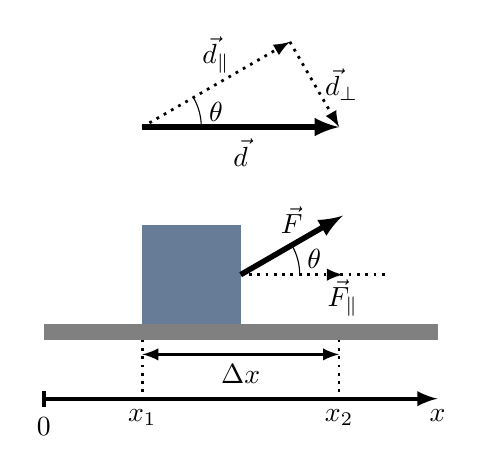
\begin{tikzpicture}[scale=1]
\tikzmath{
\L=5;
\h=0.75;
\w=0.2;
\dx=2.5;
\abox=1.25;
\th=30;
\Fm=1.5;
\Fmx=\Fm*cos(\th);
\vdx=\dx*cos(\th);
}
\scalebox{1.0}{
%axis
\draw[-latex, line width=1.5pt] (0,0) -- (\L,0) node[below]{$x$};
\draw[line width=1.5pt] (0,0.1) -- (0,-0.1) node[below]{$0$};
%floor
\fill[black!50] (0,\h) rectangle (\L,\h+\w);

\fill[color=myblue!60] (0.5*\dx,\h+\w) rectangle (0.5*\dx+\abox,\h+\w+\abox);


\draw[-latex,line width=2] (0.5*\dx+\abox,\h+\w+\abox/2) -- +(\th:\Fm) node[midway,above]{$\vec F$};
\draw[dotted,line width=1] (0.5*\dx+\abox,\h+\w+\abox/2) -- +(0:1.25*\Fm);
\draw[-latex,dotted,line width=1] (0.5*\dx+\abox,\h+\w+\abox/2) -- +(\Fmx,0) node[below=-2pt]{$\vec F_{\parallel}$};
\draw (0.5*\dx+\abox+0.75,\h+\w+\abox/2) arc(0:\th:0.75)node[midway,right]{$\theta$};

\draw[-latex,line width=2] (0.5*\dx,\h+\w+2*\abox) -- +(\dx,0) node[midway,below]{$\vec d$};
\draw[-latex,dotted,line width=1] (0.5*\dx,\h+\w+2*\abox) -- +(\th:\vdx) node[midway,above]{$\vec d_{\parallel}$};
\draw[-latex,dotted,line width=1] ($(0.5*\dx,\h+\w+2*\abox)+(\th:\vdx)$) -- (1.5*\dx,\h+\w + 2*\abox)  node[midway,right]{$\vec d_{\perp}$}; ;
\draw (0.5*\dx+0.75,\h+\w+2*\abox) arc(0:\th:0.75)node[midway,right]{$\theta$};

\draw[dotted, line width=1] (0.5*\dx,\h) -- +(0,-\h) node[below]{$x_1$};
\draw[dotted, line width=1] (1.5*\dx,\h) -- +(0,-\h) node[below]{$x_2$};

\draw[latex-latex, line width=1] (0.5*\dx,0.75*\h)--+(\dx,0) node[midway, below]{$\Delta x$};

}
\end{tikzpicture}
\captionof*{figure}{\textit{A constant force, $\vec F$, does work on the block over the displacement vector, $\vec d$.}}
\end{center}
}


%%%%%%%%%%%%%%%%%%%%%%%%%%%%%%%%


%%%%%%%%%%%%%%%%%%%%%%%%%%%%%%%%
\subsection{Work with non-constant force: 1D}
\label{subsec:workwithnonconstantforce1d}
\twocolframe{Modeling work done by a non-constant force (1D)}
{
\begin{itemize}
\item Use the component of force parallel to displacement.
\item Divide the path up into segments where the force is (almost) constant.
\item Add up the work done on each segment:
\begin{align*}
W=F_1\Delta x+ F_2\Delta x+ F_3\Delta x+\dots
\end{align*}
\item<2-> If the force changes continuously, $F(x)$, need to sum infinitesimally small segments:
\begin{align*}
W=\lim_{\Delta x \to 0}\sum F_i\Delta x=\int_{x_1}^{x_f}F(x) dx
\end{align*}
\end{itemize}

}
{
\only<1-3>{
\vspace{-1cm}
\begin{center}
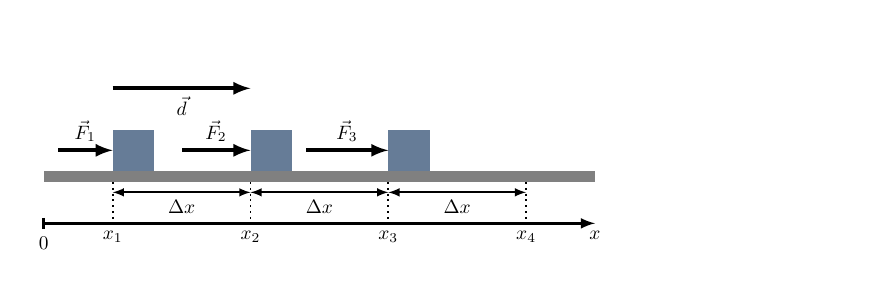
\begin{tikzpicture}[scale=1]
\tikzmath{
\L=10;
\h=0.75;
\w=0.2;
\dx=2.5;
\abox=0.75;
\Fm=1;
}
\scalebox{0.7}{
%axis
\draw[-latex, line width=1.5pt] (0,0) -- (\L,0) node[below]{$x$};
\draw[line width=1.5pt] (0,0.1) -- (0,-0.1) node[below]{$0$};
%floor
\fill[black!50] (0,\h) rectangle (\L,\h+\w);

\fill[color=myblue!60] (0.5*\dx,\h+\w) rectangle (0.5*\dx+\abox,\h+\w+\abox);
\fill[color=myblue!60] (1.5*\dx,\h+\w) rectangle (1.5*\dx+\abox,\h+\w+\abox);
\fill[color=myblue!60] (2.5*\dx,\h+\w) rectangle (2.5*\dx+\abox,\h+\w+\abox);

\draw[-latex,line width=2] (0.5*\dx,\h+\w+2*\abox) -- +(\dx,0) node[midway,below]{$\vec d$};

\draw[latex-,line width=2] (0.5*\dx,\h+\w+\abox/2) -- +(-\Fm,0) node[midway,above]{$\vec F_1$};
\draw[latex-,line width=2] (1.5*\dx,\h+\w+\abox/2) -- +(-1.25*\Fm,0) node[midway,above]{$\vec F_2$};
\draw[latex-,line width=2] (2.5*\dx,\h+\w+\abox/2) -- +(-1.5*\Fm,0) node[midway,above]{$\vec F_3$};

\draw[dotted, line width=1] (0.5*\dx,\h) -- +(0,-\h) node[below]{$x_1$};
\draw[dotted, line width=1] (1.5*\dx,\h) -- +(0,-\h) node[below]{$x_2$};
\draw[dotted, line width=1] (2.5*\dx,\h) -- +(0,-\h) node[below]{$x_3$};
\draw[dotted, line width=1] (3.5*\dx,\h) -- +(0,-\h) node[below]{$x_4$};

\draw[latex-latex, line width=1] (0.5*\dx,0.75*\h)--+(\dx,0) node[midway, below]{$\Delta x$};
\draw[latex-latex, line width=1] (1.5*\dx,0.75*\h)--+(\dx,0) node[midway, below]{$\Delta x$};
\draw[latex-latex, line width=1] (2.5*\dx,0.75*\h)--+(\dx,0) node[midway, below]{$\Delta x$};
}
\end{tikzpicture}
\captionof*{figure}{\textit{A block slides along $x$ with a force that depends on position.}}
\end{center}}
\only<3>{
\scriptsize
If $F(x)=\text{constant}$:
\begin{align*}
W=\int_{x_1}^{x_f}F(x) dx=F\int_{x_1}^{x_f} dx=F(x_f-x_1)
\end{align*}
$(x_f-x_1)$ is just the total displacement.
}

\only<4->{
\vspace{-0.2cm}
\begin{center}
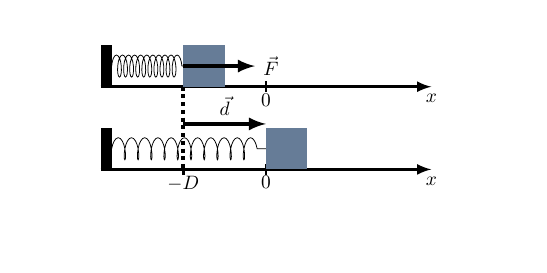
\begin{tikzpicture}[scale=1]
\tikzmath{
\L=2.;
\dx=0.75*\L;
\off=0.5;
\h=0.75;
}
\scalebox{0.7}{

\begin{scope}[shift={(0,-2*\h)}]
\draw[-latex,line width=1.5pt] (-1.5*\L,0) -- (1.5*\L,0) node[below]{$x$};
\draw[line width=1.5pt] (0,-0.1) -- (0,0.1);
\node[below] at (0,0) {$0$};

\fill (-1.5*\L,0) rectangle (-1.4*\L,\h);
\draw[decoration={aspect=0.3, segment length=2.4mm, amplitude=2mm,coil},decorate] (-1.4*\L,\h/2) -- (0,\h/2);
%\draw [latex-latex] (-1.4*\L,\h) -- (0,\h) node[midway,above]{$L_0$};
\fill[color=myblue!60] (0,0) rectangle (\h,\h);
\draw [-latex, line width=2] (-\dx,1.1*\h) -- (0,1.1*\h) node[midway,above]{$\vec d$};
 \node[below] at (-\dx,0) {$-D$};
 \draw[line width=1.5pt] (-\dx,-0.1) -- (-\dx,0.1);
\end{scope}
%%%%%%%%%%   compressed

\draw[-latex,line width=1.5pt] (-1.5*\L,0) -- (1.5*\L,0) node[below]{$x$};
\draw[line width=1.5pt] (0,-0.1) -- (0,0.1);
\node[below] at (0,0) {$0$};

\fill (-1.5*\L,0) rectangle (-1.4*\L,\h);
\draw[decoration={aspect=0.3, segment length=1.1mm, amplitude=2mm,coil},decorate] (-1.4*\L,\h/2) -- (-\dx,\h/2);

\fill[color=myblue!60] (-\dx,0) rectangle (-\dx+\h,\h);
\draw[line width=2, -latex] (-\dx,\h/2) -- +(1.3,0) node[right] {$\vec F$};
\draw[dotted,line width=2] (-\dx,0) -- +(0,-2*\h);

}
\end{tikzpicture}
\vspace{-0.2cm}
\captionof*{figure}{\textit{A spring does \textbf{positive} work on a block over a total displacement, $\vec d$, from $x=-D$ to $x=0$. The spring force depends on position, $F(x)=-kx$.}}
\end{center}
}
\only<5>{
\scriptsize
\begin{align*}
W&=\int_{x_1}^{x_f}F(x) dx=\int_{-D}^0 (-kx)dx=\left[-\frac{1}{2}kx^2 \right]_{-D}^0\\
&=\frac{1}{2}kD^2\quad\text{}
\end{align*}
The work done by a spring over a distance, $D$.
}
}
%%%%%%%%%%%%%%%%%%%%%%%%%%%%%%%%





%%%%%%%%%%%%%%%%%%%%%%%%%%%%%%%

\section{Work in nD}
\label{sec:workinnd}
\title{Work in nD}
\institute{Work \& Energy}
\author{\insertsubsection}


%%%%%%%%%%%%%%%%%%%%%%%%%
\begin{frame}
\titlepage
\thispagestyle{empty}
\end{frame}

%%%%%%%%%%%%%%%%%%%%%%%%










%%%%%%%%%%%%%%%%%%%%%%%%%%%%%%%%
\subsection{1D vs nD}
\label{subsec:1dvsnd}
\twocolframesf{Work in ND}
{
\begin{itemize}
\item Defined work, a scalar quantity, as a first step towards using scalars to describe the world instead of vectors:
\begin{align*}
W=\vec F\cdot \vec d
\end{align*}
\item The work done by a force is a measure of how much that force contributes to changing the speed of an object.
\item In general, the displacement may not be one-dimensional:
\begin{align*}
W=\vec F \cdot \vec d_1+\vec F \cdot \vec d_2+\vec F \cdot \vec d_3+
\end{align*}
\end{itemize}
}
{\vspace{-1.5cm}
%%%%%%%%%%% block with force
\begin{center}
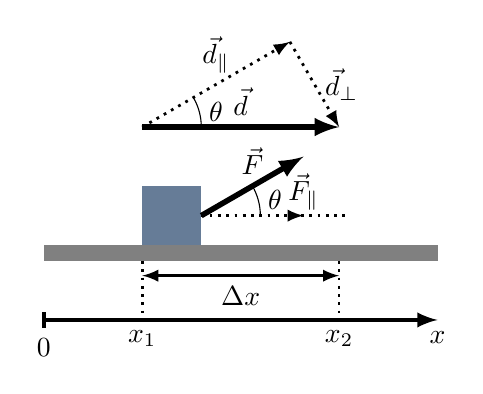
\begin{tikzpicture}[scale=1]
\tikzmath{
\L=5;
\h=0.75;
\w=0.2;
\dx=2.5;
\abox=0.75;
\th=30;
\Fm=1.5;
\Fmx=\Fm*cos(\th);
\vdx=\dx*cos(\th);
}
\scalebox{1.0}{
%axis
\draw[-latex, line width=1.5pt] (0,0) -- (\L,0) node[below]{$x$};
\draw[line width=1.5pt] (0,0.1) -- (0,-0.1) node[below]{$0$};
%floor
\fill[black!50] (0,\h) rectangle (\L,\h+\w);

\fill[color=myblue!60] (0.5*\dx,\h+\w) rectangle (0.5*\dx+\abox,\h+\w+\abox);


\draw[-latex,line width=2] (0.5*\dx+\abox,\h+\w+\abox/2) -- +(\th:\Fm) node[midway,above]{$\vec F$};
\draw[dotted,line width=1] (0.5*\dx+\abox,\h+\w+\abox/2) -- +(0:1.25*\Fm);
\draw[-latex,dotted,line width=1] (0.5*\dx+\abox,\h+\w+\abox/2) -- +(\Fmx,0) node[above=-2pt]{$\vec F_{\parallel}$};
\draw (0.5*\dx+\abox+0.75,\h+\w+\abox/2) arc(0:\th:0.75)node[midway,right]{$\theta$};

\draw[-latex,line width=2] (0.5*\dx,\h+\w+2*\abox) -- +(\dx,0) node[midway,above]{$\vec d$};
\draw[-latex,dotted,line width=1] (0.5*\dx,\h+\w+2*\abox) -- +(\th:\vdx) node[midway,above]{$\vec d_{\parallel}$};
\draw[-latex,dotted,line width=1] ($(0.5*\dx,\h+\w+2*\abox)+(\th:\vdx)$) -- (1.5*\dx,\h+\w + 2*\abox)  node[midway,right]{$\vec d_{\perp}$}; ;
\draw (0.5*\dx+0.75,\h+\w+2*\abox) arc(0:\th:0.75)node[midway,right]{$\theta$};

\draw[dotted, line width=1] (0.5*\dx,\h) -- +(0,-\h) node[below]{$x_1$};
\draw[dotted, line width=1] (1.5*\dx,\h) -- +(0,-\h) node[below]{$x_2$};

\draw[latex-latex, line width=1] (0.5*\dx,0.75*\h)--+(\dx,0) node[midway, below]{$\Delta x$};

}
\end{tikzpicture}
%\captionof*{figure}{\textit{A constant force, $\vec F$, does work on the block over the displacement vector, $\vec d$.}}
\end{center}

%%%%%%% top view of ND motion:
\begin{center}
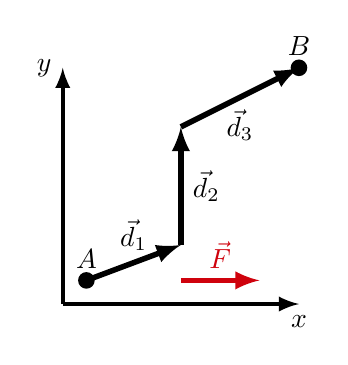
\begin{tikzpicture}[scale=1]
\tikzmath{
\L=3;
}
\scalebox{1.0}{
%axis
\coordinate (P1) at (0.1*\L,0.1*\L);
\coordinate (P2) at (0.5*\L,0.25*\L);
\coordinate (P3) at (0.5*\L,0.75*\L);
\coordinate (P4) at (1*\L,1*\L);

\fill (P1) circle(3pt);
\fill (P4) circle(3pt);
\draw[-latex, line width=1.5pt] (0,0) -- (0,\L) node[left]{$y$};
\draw[-latex, line width=1.5pt] (0,0) -- (\L,0) node[below]{$x$};

\draw[-latex, line width=2.pt, color=myred] (0.5*\L,0.1*\L) -- +(1,0) node[midway,above]{$\vec F$};

\draw[-latex, line width=2.pt] (P1) node[above]{$A$} -- (P2) node[midway,above]{$\vec d_1$};
\draw[-latex, line width=2.pt] (P2) -- (P3)node[midway,right]{$\vec d_2$};
\draw[-latex, line width=2.pt] (P3) -- (P4)node[midway,below]{$\vec d_3$} node[above]{$B$};


}
\end{tikzpicture}
%\captionof*{figure}{\textit{A constant force, $\vec F$, does work on the block over the displacement vector, $\vec d$.}}
\end{center}
}


%%%%%%%%%%%%%%%%%%%%%%%%%%%%%%%%

%%%%%%%%%%%%%%%%%%%%%%%%%%%%%%%%
\twocolframe{Recall 1D case}
{
\begin{itemize}
\item When force changes as a function of position, we must break up the motion into infinitesimal segments and use an integral to calculate the work:
\begin{align*}
W=\lim_{\Delta x \to 0}\sum F_i\Delta x=\int_{x_1}^{x_f}F(x) dx
\end{align*}
\item The net work done by a force can depend on the path taken between $x_1$ and $x_f$:
\begin{itemize}
\item For friction, it matters.
\item For a spring force, it doesn't matter.

\end{itemize}

\end{itemize}
}
{
\vspace{-2cm}
%$%%%%%%%%%%%%%% block on a line
\begin{center}
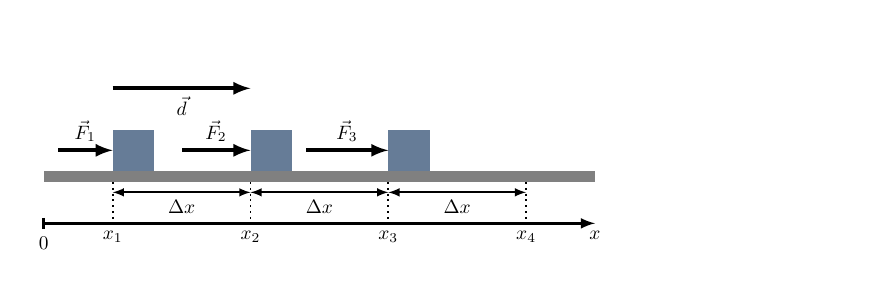
\begin{tikzpicture}[scale=1]
\tikzmath{
\L=10;
\h=0.75;
\w=0.2;
\dx=2.5;
\abox=0.75;
\Fm=1;
}
\scalebox{0.7}{
%axis
\draw[-latex, line width=1.5pt] (0,0) -- (\L,0) node[below]{$x$};
\draw[line width=1.5pt] (0,0.1) -- (0,-0.1) node[below]{$0$};
%floor
\fill[black!50] (0,\h) rectangle (\L,\h+\w);

\fill[color=myblue!60] (0.5*\dx,\h+\w) rectangle (0.5*\dx+\abox,\h+\w+\abox);
\fill[color=myblue!60] (1.5*\dx,\h+\w) rectangle (1.5*\dx+\abox,\h+\w+\abox);
\fill[color=myblue!60] (2.5*\dx,\h+\w) rectangle (2.5*\dx+\abox,\h+\w+\abox);

\draw[-latex,line width=2] (0.5*\dx,\h+\w+2*\abox) -- +(\dx,0) node[midway,below]{$\vec d$};

\draw[latex-,line width=2] (0.5*\dx,\h+\w+\abox/2) -- +(-\Fm,0) node[midway,above]{$\vec F_1$};
\draw[latex-,line width=2] (1.5*\dx,\h+\w+\abox/2) -- +(-1.25*\Fm,0) node[midway,above]{$\vec F_2$};
\draw[latex-,line width=2] (2.5*\dx,\h+\w+\abox/2) -- +(-1.5*\Fm,0) node[midway,above]{$\vec F_3$};

\draw[dotted, line width=1] (0.5*\dx,\h) -- +(0,-\h) node[below]{$x_1$};
\draw[dotted, line width=1] (1.5*\dx,\h) -- +(0,-\h) node[below]{$x_2$};
\draw[dotted, line width=1] (2.5*\dx,\h) -- +(0,-\h) node[below]{$x_3$};
\draw[dotted, line width=1] (3.5*\dx,\h) -- +(0,-\h) node[below]{$x_4$};

\draw[latex-latex, line width=1] (0.5*\dx,0.75*\h)--+(\dx,0) node[midway, below]{$\Delta x$};
\draw[latex-latex, line width=1] (1.5*\dx,0.75*\h)--+(\dx,0) node[midway, below]{$\Delta x$};
\draw[latex-latex, line width=1] (2.5*\dx,0.75*\h)--+(\dx,0) node[midway, below]{$\Delta x$};
}
\end{tikzpicture}
\captionof*{figure}{\textit{A block slides along $x$ with a force that depends on position.}}
\end{center}
%%%%%%%%%%%%%%%% spring
\begin{center}
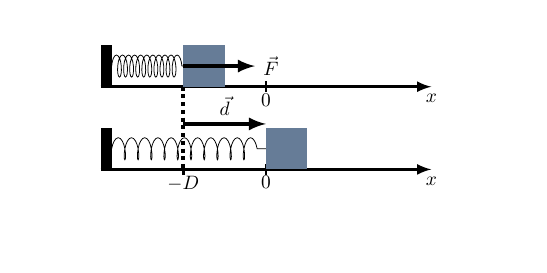
\begin{tikzpicture}[scale=1]
\tikzmath{
\L=2.;
\dx=0.75*\L;
\off=0.5;
\h=0.75;
}
\scalebox{0.7}{

\begin{scope}[shift={(0,-2*\h)}]
\draw[-latex,line width=1.5pt] (-1.5*\L,0) -- (1.5*\L,0) node[below]{$x$};
\draw[line width=1.5pt] (0,-0.1) -- (0,0.1);
\node[below] at (0,0) {$0$};

\fill (-1.5*\L,0) rectangle (-1.4*\L,\h);
\draw[decoration={aspect=0.3, segment length=2.4mm, amplitude=2mm,coil},decorate] (-1.4*\L,\h/2) -- (0,\h/2);
%\draw [latex-latex] (-1.4*\L,\h) -- (0,\h) node[midway,above]{$L_0$};
\fill[color=myblue!60] (0,0) rectangle (\h,\h);
\draw [-latex, line width=2] (-\dx,1.1*\h) -- (0,1.1*\h) node[midway,above]{$\vec d$};
 \node[below] at (-\dx,0) {$-D$};
 \draw[line width=1.5pt] (-\dx,-0.1) -- (-\dx,0.1);
\end{scope}
%%%%%%%%%%   compressed

\draw[-latex,line width=1.5pt] (-1.5*\L,0) -- (1.5*\L,0) node[below]{$x$};
\draw[line width=1.5pt] (0,-0.1) -- (0,0.1);
\node[below] at (0,0) {$0$};

\fill (-1.5*\L,0) rectangle (-1.4*\L,\h);
\draw[decoration={aspect=0.3, segment length=1.1mm, amplitude=2mm,coil},decorate] (-1.4*\L,\h/2) -- (-\dx,\h/2);

\fill[color=myblue!60] (-\dx,0) rectangle (-\dx+\h,\h);
\draw[line width=2, -latex] (-\dx,\h/2) -- +(1.3,0) node[right] {$\vec F$};
\draw[dotted,line width=2] (-\dx,0) -- +(0,-2*\h);

}
\end{tikzpicture}
\captionof*{figure}{\textit{A spring does positive work on a block over a total displacement, $\vec d$, from $x=-D$ to $x=0$.}}
\end{center}
}


%%%%%%%%%%%%%%%%%%%%%%%%%%%%%%%%
\twocolframesf{In multiple dimensions}
{
\begin{itemize}
\item Force can depend on position (x,y,z) $\rightarrow$ $\vec F=\vec F(\vec r)$, where $\vec r$, is the position of the object.
\item A infinitesimal segment is not necessarily parallel to the $x,y,z$ axis, use $d\vec l$.
\item We write work as:
\begin{align*}
W=\int_A^B \vec F(\vec r) \cdot d\vec l
\end{align*}
\item Where $d\vec l$ is an infinitesimal segment, tangent to the path
\end{itemize}
}
{
\begin{center}
\begin{tikzpicture}[%
%https://tex.stackexchange.com/questions/25928/how-to-draw-tangent-line-of-an-arbitrary-point-on-a-path-in-tikz
        tangent/.style={
        decoration={
            markings,% switch on markings
            mark=
                at position ####1
                with
                {
                    \coordinate (tangent point-\pgfkeysvalueof{/pgf/decoration/mark info/sequence number}) at (0pt,0pt);
                    \coordinate (tangent unit vector-\pgfkeysvalueof{/pgf/decoration/mark info/sequence number}) at (1,0pt);
                    \coordinate (tangent orthogonal unit vector-\pgfkeysvalueof{/pgf/decoration/mark info/sequence number}) at (0pt,1);
                }
        },
        postaction=decorate
    },
    use tangent/.style={
        shift=(tangent point-####1),
        x=(tangent unit vector-####1),
        y=(tangent orthogonal unit vector-####1)
    },
    use tangent/.default=1
    ]
\tikzmath{
}

\scalebox{1.0}{

 \coordinate (P1) at (0.2,0.5);
 \coordinate (P2) at (1.75,2); %used to make the path squiggly
 \coordinate (P3) at (3.75,2.5);
 \coordinate (P3x) at ($(0,0)!(P3)!(1,0)$);
 \coordinate (P1P3) at ($(P3)!(P1)!(P3x)$);
 
 \draw[-latex, line width=1.5pt] (0,0) -- (4.5,0) node[below]{$x$}; 
 \draw[-latex, line width=1.5pt] (0,0) -- (0,3) node[left]{$y$}; 
 
 \fill (P1) circle(2pt) node[above]{$A$};;
 \fill (P3) circle(2pt) node[above]{$B$};;
 
  
 %The path with tangent coordinates calculated
 \draw[tangent=0.25,tangent=0.45,tangent=0.65, tangent=0.85,  line width=1pt] (P1) to [out=10,in=190] (P2) to [out=10,in=260] (P3);
 
 \draw [myred, -latex, line width=1.5, use tangent=2] (0,0) -- (0.5,0) node[above]{$d\vec l$};
 \draw [ -latex, line width=1.5, use tangent=2] (0,0) -- +(-60:1) node[right]{$\vec F(\vec r)$}; 
 \draw [ -latex, line width=1.5, use tangent=1] (0,0) -- +(-80:0.75) node[below]{$\vec F(\vec r)$}; 
 \draw [ -latex, line width=1.5, use tangent=3] (0,0) -- +(60:1.25) node[above]{$\vec F(\vec r)$}; 
}
\end{tikzpicture}
\captionof*{figure}{\textit{A position-dependent force, $\vec F(\vec r)$, does work along an arbitrary path.}}
\end{center}
}


%%%%%%%%%%%%%%%%%%%%%%%%%%%%%%%%

%%%%%%%%%%%%%%%%%%%%%%%%%%%%%%%%
\subsection{Path integrals}
\label{subsec:pathinegrals}
\twocolframesf{Path integrals}
{
\begin{itemize}
\item In general, the value of the integral will depend on what path you take between points $A$ and $B$ (think friction doing work).
\item This is different than ``normal'' integrals which only depend on the end points (you just evaluate the anti-derivative at the end points).
\item There are some forces (i.e. some functions ) for which the work done ultimately does not depend on the path taken, like gravity, which we will discuss next week.
\item \textbf{In general, it does depend on the path, and it’s difficult to calculate! We want to avoid doing this integral if we can!}
\end{itemize}
}
{
\begin{center}
\begin{tikzpicture}[%
%https://tex.stackexchange.com/questions/25928/how-to-draw-tangent-line-of-an-arbitrary-point-on-a-path-in-tikz
        tangent/.style={
        decoration={
            markings,% switch on markings
            mark=
                at position ####1
                with
                {
                    \coordinate (tangent point-\pgfkeysvalueof{/pgf/decoration/mark info/sequence number}) at (0pt,0pt);
                    \coordinate (tangent unit vector-\pgfkeysvalueof{/pgf/decoration/mark info/sequence number}) at (1,0pt);
                    \coordinate (tangent orthogonal unit vector-\pgfkeysvalueof{/pgf/decoration/mark info/sequence number}) at (0pt,1);
                }
        },
        postaction=decorate
    },
    use tangent/.style={
        shift=(tangent point-####1),
        x=(tangent unit vector-####1),
        y=(tangent orthogonal unit vector-####1)
    },
    use tangent/.default=1
    ]
\tikzmath{
}

\scalebox{1.0}{

 \coordinate (P1) at (0.2,0.5);
 \coordinate (P2) at (1.75,2); %used to make the path squiggly
 \coordinate (P3) at (3.75,2.5);
 \coordinate (P3x) at ($(0,0)!(P3)!(1,0)$);
 \coordinate (P1P3) at ($(P3)!(P1)!(P3x)$);
 
 \draw[-latex, line width=1.5pt] (0,0) -- (4.5,0) node[below]{$x$}; 
 \draw[-latex, line width=1.5pt] (0,0) -- (0,3) node[left]{$y$}; 
 
 \fill (P1) circle(2pt) node[above]{$A$};;
 \fill (P3) circle(2pt) node[above]{$B$};;
 
  
 %The path with tangent coordinates calculated
 \draw[tangent=0.25,tangent=0.45,tangent=0.65, tangent=0.85,  line width=1pt] (P1) to [out=10,in=190] (P2) to [out=10,in=260] (P3);
 
 \draw [myred, -latex, line width=1.5, use tangent=2] (0,0) -- (0.5,0) node[above]{$d\vec l$};

}
\end{tikzpicture}
\captionof*{figure}{\textit{An arbitrary path over which we may need to calculate a path integral.}}
\end{center}
}

%%%%%%%%%%%%%%%%%%%%%%%%%%%%%%%%
\subsection{Work from gravity on a pendulum}
\label{subsec:workfromgravityonpendulum}
\twocolframesf{Example: Work done by gravity on pendulum}
{
\scriptsize
\begin{itemize}
\item We want the work done by gravity along the arc:
\begin{align*}
W=\int_A^B \vec F_g\cdot d\vec l
\end{align*}
\item<2-> At some angle, $\theta$:
\begin{align*}
d\vec l &= dl(\cos\theta\hat x-\sin\theta\hat y)\\
\vec F_g&=-mg\hat y\\
\therefore \vec F_g\cdot d\vec l &=mg\sin\theta dl
\end{align*}
\item<3-> Noting that $dl=-Ld\theta$ ($d\theta$ is in the direction of increasing $\theta$):
\begin{align*}
W&=\int_A^B \vec F_g\cdot d\vec l=\int_{\theta_0}^0-mg\sin\theta L d\theta=mgL(1-\cos\theta_0)\\
&=mgh
\end{align*}
\end{itemize}

}
{
\begin{center}
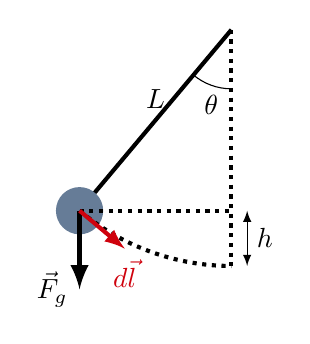
\begin{tikzpicture}[scale=1]
\tikzmath{
\L=3.;
\R=0.3;
\th=40;
\vg=1;
\Ly=\L*cos(\th);
}
\scalebox{1.0}{
%pendulum

\draw[line width = 1.5pt] (0,0) -- (270-\th:\L) node[midway,above]{$L$};
\fill[color=myblue!60] (270-\th:\L) circle(\R); 
\draw[-latex, line width= 2pt](270-\th:\L) --+(0,-\vg) node[left]{$\vec F_g$};

\draw[dotted, line width = 1.5pt] (0,0) -- (270:\L);
\draw[dotted, line width = 1.5pt] (270-\th:\L) arc (270-\th:270:\L);
\draw (270-\th:0.75) arc (270-\th:270:0.75) node[midway,below]{$\theta$};
\draw[dotted, line width = 1.5pt] (270-\th:\L) -- (0,-\Ly);
\draw[latex-latex] (0.2,-\L) -- (0.2,-\Ly) node[midway,right]{$h$};
\draw[-latex,color=myred, line width = 1.5pt] (270-\th:\L) -- +(-\th:0.75) node[below]{$d\vec l$};
}
\end{tikzpicture}
\captionof*{figure}{\textit{Gravity does work on a pendulum as it swings from $\theta=\theta_0$ to $\theta=0$. The force is constant along the path, but the path is not a straight line.}}
\end{center}

}


%%%%%%%%%%%%%%%%%%%%%%%%%%%%%%%%









%%%%%%%%%%%%%%%%%%%%%%%%%%%%%%%%

\section{Work-Energy Theorem}
\label{sec:workenergytheorem}
\title{Work-Energy Theorem}
\institute{Work \& Energy}
\author{\insertsubsection}


%%%%%%%%%%%%%%%%%%%%%%%%%
\begin{frame}
\titlepage
\thispagestyle{empty}
\end{frame}

%%%%%%%%%%%%%%%%%%%%%%%%%%%%%%%%














%%%%%%%%%%%%%%%%%%%%%%%%%%%%%%%%
\subsection{Net work}
\label{subsec:network}
\twocolframesf{Work, in general}
{
\begin{align*}
W=\int_A^B \vec F(\vec r)\cdot d\vec r
\end{align*}
\begin{itemize}
\item Force can change magnitude and direction depending on position, $\vec F(\vec r)$.
\item Need to define work as a ``path integral'', as it depends on the path taken.
\item For example, to calculate the work done by friction in moving a crate along the floor, we summed the work done on each segment (path 2):
\begin{align*}
W=\vec f_1\cdot \vec d_1+\vec f_2 \cdot \vec d_2
\end{align*}
\end{itemize}
}
{
\begin{center}
\begin{tikzpicture}[%
%https://tex.stackexchange.com/questions/25928/how-to-draw-tangent-line-of-an-arbitrary-point-on-a-path-in-tikz
        tangent/.style={
        decoration={
            markings,% switch on markings
            mark=
                at position ####1
                with
                {
                    \coordinate (tangent point-\pgfkeysvalueof{/pgf/decoration/mark info/sequence number}) at (0pt,0pt);
                    \coordinate (tangent unit vector-\pgfkeysvalueof{/pgf/decoration/mark info/sequence number}) at (1,0pt);
                    \coordinate (tangent orthogonal unit vector-\pgfkeysvalueof{/pgf/decoration/mark info/sequence number}) at (0pt,1);
                }
        },
        postaction=decorate
    },
    use tangent/.style={
        shift=(tangent point-####1),
        x=(tangent unit vector-####1),
        y=(tangent orthogonal unit vector-####1)
    },
    use tangent/.default=1
    ]
\tikzmath{
}

\scalebox{1.0}{

 \coordinate (P1) at (0.2,0.5);
 \coordinate (P2) at (1.75,2); %used to make the path squiggly
 \coordinate (P3) at (3.75,2.5);
 \coordinate (P3x) at ($(0,0)!(P3)!(1,0)$);
 \coordinate (P1P3) at ($(P3)!(P1)!(P3x)$);
 
 \draw[-latex, line width=1.5pt] (0,0) -- (4.5,0) node[below]{$x$}; 
 \draw[-latex, line width=1.5pt] (0,0) -- (0,3) node[left]{$y$}; 
 
 \fill (P1) circle(2pt) node[above]{$A$};;
 \fill (P3) circle(2pt) node[above]{$B$};;
 
  
 %The path with tangent coordinates calculated
 \draw[tangent=0.25,tangent=0.45,tangent=0.65, tangent=0.85,  line width=1pt] (P1) to [out=10,in=190] (P2) to [out=10,in=260] (P3);
 
 \draw [myred, -latex, line width=1.5, use tangent=2] (-0.25,0) -- (0.25,0) node[above]{$d\vec l$};
 %\draw [ -latex, line width=1.5, use tangent=2] (0,0) -- +(-60:1) node[right]{$\vec F(\vec r)$}; 
 \draw [ -latex, line width=1.5, use tangent=1] (0,0) -- +(-80:0.75) node[below]{$\vec F(\vec r)$}; 
 %\draw [ -latex, line width=1.5, use tangent=3] (0,0) -- +(60:1.25) node[above]{$\vec F(\vec r)$}; 
 
 \begin{scope}[shift={(0,-3.5)}]
 
 \coordinate (A) at (0.75,0.5);
 \coordinate (B) at (3.75,2.5);
 
 
 \draw[-latex, line width=1.5pt] (0,0) -- (4.5,0) node[below]{$x$}; 
 \draw[-latex, line width=1.5pt] (0,0) -- (0,3) node[left]{$y$}; 

 \fill (A) circle(2pt) node[right]{$A(x_A,y_A)$};
 \fill (B) circle(2pt) node[above]{$B(x_B,y_B)$};
 
 \draw[dashed, line width=1.5] (A)--(B) node[midway,right=5pt]{path 1};
 
 \draw[-latex, color=myred, line width=1.5pt] (A)-- +(0,2.0)node[midway,left]{$\vec d_1$} node[above]{path 2};
 \draw[latex-, color=myred, line width=1.5pt] (B)-- +(-3,0) node[midway,above]{$\vec d_2$};
 
 \draw[latex-, line width=3] (1,1) -- +(0,1) node[midway, right]{$\vec f_1$};
 \draw[-latex, line width=3] (2.5,2.25) -- +(-1,0) node[midway, below]{$\vec f_2$};
 
 
 \end{scope} 
 
}
\end{tikzpicture}
\captionof*{figure}{\textit{Work is a path integral.}}
\end{center}

}


%%%%%%%%%%%%%%%%%%%%%%%%%%%%%%%%


%%%%%%%%%%%%%%%%%%%%%%%%%%%%%%%%
\begin{frame}{Net work done}
\begin{itemize}
\item If multiple forces are exerted on an object, as it moves, they can each do work.
\item The net work done on the object is the sum of the work done by each force exerted on the object:
\begin{align*}
W^{net}=\vec F_1\cdot \vec d+\vec F_2 \cdot \vec d+\vec F_3 \cdot \vec d+\dots
\end{align*}
\item Very easy to show that this is equivalent to:
\begin{align*}
W^{net}=(\vec F_1+\vec F_2+\vec F_3+\dots)\cdot \vec d=\vec F^{net}\cdot \vec d
\end{align*}
\end{itemize}
That is, the net work done on the object is the same as the work done by the net force.
\end{frame}


%%%%%%%%%%%%%%%%%%%%%%%%%%%%%%%%


%%%%%%%%%%%%%%%%%%%%%%%%%%%%%%%%
\subsection{Work-energy theorem}
\label{subsec:workenergytheorem}
\twocolframesf{Work-Energy theorem}
{\scriptsize
\begin{itemize}
\item<1-> In general, the \textbf{net} work done on an object can be written as:
\begin{align*}
W^{net}=\int_A^B\vec F^{net}(\vec r) \cdot d\vec l
\end{align*}
\item<2-> Using Newton’s Second Law:
\begin{align*}
F^{net} &= m\vec a =m\frac{d\vec v}{dt}\\
W^{net} &=\int_A^B m\frac{d\vec v}{dt}\cdot d\vec l\\
\only<3->{
&=m\int_A^B \frac{d\vec v}{dt}\cdot d\vec l=m\int_A^B d\vec v\cdot \frac{d\vec l}{dt}\\
}
\only<4->{
&=m\int_A^B d\vec v\cdot \vec v=m\int_A^B v dv\\
}
\only<5->{
&=\frac{1}{2}mv^2_B-\frac{1}{2}mv_A^2
}
\end{align*}
\end{itemize}
}
{
\begin{center}
\begin{tikzpicture}[%
%https://tex.stackexchange.com/questions/25928/how-to-draw-tangent-line-of-an-arbitrary-point-on-a-path-in-tikz
        tangent/.style={
        decoration={
            markings,% switch on markings
            mark=
                at position ####1
                with
                {
                    \coordinate (tangent point-\pgfkeysvalueof{/pgf/decoration/mark info/sequence number}) at (0pt,0pt);
                    \coordinate (tangent unit vector-\pgfkeysvalueof{/pgf/decoration/mark info/sequence number}) at (1,0pt);
                    \coordinate (tangent orthogonal unit vector-\pgfkeysvalueof{/pgf/decoration/mark info/sequence number}) at (0pt,1);
                }
        },
        postaction=decorate
    },
    use tangent/.style={
        shift=(tangent point-####1),
        x=(tangent unit vector-####1),
        y=(tangent orthogonal unit vector-####1)
    },
    use tangent/.default=1
    ]
\tikzmath{
}

\scalebox{1}{

 \coordinate (P1) at (0.2,0.5);
 \coordinate (P2) at (1.75,2); %used to make the path squiggly
 \coordinate (P3) at (3.75,2.5);
 \coordinate (P3x) at ($(0,0)!(P3)!(1,0)$);
 \coordinate (P1P3) at ($(P3)!(P1)!(P3x)$);
 
 \draw[-latex, line width=1.5pt] (0,0) -- (4.5,0) node[below]{$x$}; 
 \draw[-latex, line width=1.5pt] (0,0) -- (0,3) node[left]{$y$}; 
 
 \fill (P1) circle(2pt) node[above]{$A$};;
 \fill (P3) circle(2pt) node[above]{$B$};;
 
  
 %The path with tangent coordinates calculated
 \draw[tangent=0.25,tangent=0.45,tangent=0.65, tangent=0.85,  line width=1pt] (P1) to [out=10,in=190] (P2) to [out=10,in=260] (P3);
 
 \draw [myred, -latex, line width=1.5, use tangent=2] (-0.25,0) -- (0.25,0) node[above]{$\vec v = \frac{d\vec l}{dt}$};

}
\end{tikzpicture}
\captionof*{figure}{\textit{Instantaneous velocity, $\vec v$ is parallel to displacement, $d\vec l$.}}
\end{center}

}


%%%%%%%%%%%%%%%%%%%%%%%%%%%%%%%%
\begin{frame}{Work-Energy Theorem}
\begin{itemize}
\item Introduce ``Kinetic energy'':
\begin{align*}
K(v)=\frac{1}{2}mv^2
\end{align*}
\item The net work done on an object is the change in kinetic energy (final – initial)
\begin{align*}
W^{net} = \Delta K = K_B-K_A
\end{align*}
\item Now, we have a way to build models using scalar quantities (next week, we’ll introduce potential energy as a way to calculate work without using force vectors or path integrals). Note the connection between dynamics ($W$) and kinematics ($K$), just like Newton's Second Law (not surprising, since this came from Newton's Second Law!).
\end{itemize}
\end{frame}


%%%%%%%%%%%%%%%%%%%%%%%%%%%%%%%%


%%%%%%%%%%%%%%%%%%%%%%%%%%%%%%%%
\subsection{Power}
\label{subsec:power}
\begin{frame}{Power}
\begin{itemize}
\item Power is the rate at which work is being done.
\item If a force does work, $\Delta W$, in an amount of time, $\Delta t$, it did work with an average power:
\begin{align*}
P=\frac{\Delta W}{\Delta t}
\end{align*}
\item If the work done changes as a function of time, then we take the limit of $\Delta t\to 0$ to get the instantaneous power:
\begin{align*}
P=\frac{d W}{d t}
\end{align*}
\item Power is the rate at which a force changes the kinetic energy of an object (if it is the only force doing work) $\rightarrow$ think of this as the rate at which (kinetic) energy is being ``given/removed'' to/from the object.
\end{itemize}
\end{frame}


%%%%%%%%%%%%%%%%%%%%%%%%%%%%%%%%



%%%%%%%%%%%%%%%%%%%%%%%%%%%%%%%%



%%%%%%%%%%%%%%%%%%%%%%%%%%%%%%%%



%%%%%%%%%%%%%%%%%%%%%%%%%%%%%%%%



%%%%%%%%%%%%%%%%%%%%%%%%%%%%%%%%



%%%%%%%%%%%%%%%%%%%%%%%%%%%%%%%%



%%%%%%%%%%%%%%%%%%%%%%%%%%%%%%%%



%%%%%%%%%%%%%%%%%%%%%%%%%%%%%%%%



%%%%%%%%%%%%%%%%%%%%%%%%%%%%%%%%



%%%%%%%%%%%%%%%%%%%%%%%%%%%%%%%%



%%%%%%%%%%%%%%%%%%%%%%%%%%%%%%%%



%%%%%%%%%%%%%%%%%%%%%%%%%%%%%%%%



%%%%%%%%%%%%%%%%%%%%%%%%%%%%%%%%



%%%%%%%%%%%%%%%%%%%%%%%%%%%%%%%%



%%%%%%%%%%%%%%%%%%%%%%%%%%%%%%%%






\end{document}